% A simple graph with straight and bend arrows and loops
% Stefan Kottwitz
\documentclass{article}
\usepackage{tikz}
%\usetikzlibrary{arrows}
\begin{document}

%%% 3.1.1. %%%
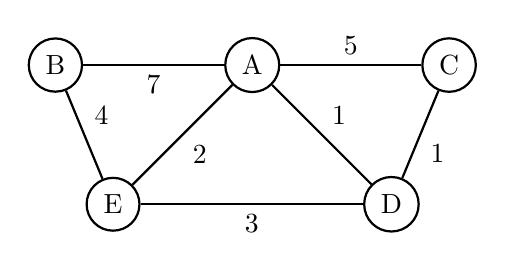
\begin{tikzpicture}[-,
					%>=stealth',
					%shorten >=1pt,
					auto,
					node distance=2.5cm,
					thick,
					main node/.style={circle,draw}]

  \node[main node] (A) {A};
  \node[main node] (B) [left of=A] {B};
  \node[main node] (C) [right of=A] {C};
  \node[main node] (D) [below right of=A] {D};
  \node[main node] (E) [below left of=A] {E};
  
  \path[every node/.style={}]
    (A) edge node {7} (B)
        edge node {5} (C)
        edge node {1} (D)
        edge node {2} (E)
    (B) edge node {4} (E)
  	(C) edge node {1} (D)
  	(D) edge node {3} (E);
\end{tikzpicture}

\begin{table}
\begin{tabular}{c|c}
Node & Distance \\
\hline
B & 7\\
C & 5\\
D & 1\\
E & 2
\end{tabular}
\caption{The first distance table of Node A}
\end{table}

\begin{tabular}{c|c}
Node & Distance \\ \hline A & 7 \\ E & 4
\end{tabular}

\begin{tabular}{c|c}
Node & Distance \\ \hline A & 5 \\ D & 1
\end{tabular}

\begin{tabular}{c|c}
Node & Distance \\ \hline A & 1 \\ C & 1 \\ E & 3
\end{tabular}

\begin{tabular}{c|c}
Node & Distance \\ \hline A & 2 \\ B & 4 \\ D & 3
\end{tabular}

In der ersten Welle der Update-Nachrichten wird jeder Knoten alle seine Nachbarknoten über alle Knoten informieren, die er erreichen kann.
%%% 3.1.2 %%%

\end{document}
